\documentclass[11pt]{article}
\usepackage[a4paper,margin=1in]{geometry}
\usepackage[T1]{fontenc}
\usepackage{amsmath,amssymb,booktabs,array}
\usepackage{graphicx}
\usepackage[authoryear,round]{natbib}
\usepackage{url}
\usepackage[hidelinks]{hyperref}
\title{Do Mitigation Methods for Class Imbalance\\Improve on Temperature Scaling?}
\author{Yannik Queisler}
\date{October 28, 2026}

\begin{document}
\raggedbottom
\widowpenalty=10000
\clubpenalty=10000
\setlength{\emergencystretch}{2em}
\maketitle
\begin{abstract}
\noindent Methods that mitigate class imbalance also change how confident a classifier is. Earlier studies trained eight such methods on two histopathology datasets, BRACS and TCGA-UT, each with two foundation-model encoders. After temperature scaling, which divides all logits by one constant fitted on validation data, the probability quality of every method looked similar to that of plain cross-entropy (CE) training. This report tests whether any method improves on temperature-scaled CE, using the stored test predictions and no new training. The endpoint is the paired difference in temperature-scaled negative log-likelihood (NLL) at an imbalance ratio of 100, and a gain counts as meaningful from 0.05 nats. The claim that no method improves on temperature scaling is not confirmed. The curriculum of data augmentation (CUDA) improves meaningfully on TCGA-UT with both encoders, by 0.09 and 0.15 nats. Its calibration error after scaling is no lower than that of the other methods, so this gain reflects better discrimination rather than better calibration. The other methods lie within 0.06 nats of scaled CE; about half of these comparisons are inconclusive, because of wide intervals on BRACS and small but consistent gains on TCGA-UT. Without temperature scaling, no method except CUDA on TCGA-UT comes close to scaled CE. Mitigation methods therefore do not replace temperature scaling, and after scaling they add little to it.
\end{abstract}

\section{Motivation}
\label{sec:motivation}
The mitigation studies trained eight methods against class imbalance, each together with a low-rank adaptation (LoRA) of the encoder \citep{queisler2026mitigationMethods}. They covered BRACS and TCGA-UT with Virchow2 \citep{zimmermann2024virchow2,queisler2026mitigationBracs,queisler2026mitigationTcga} and repeated both with UNI2-h \citep{mahmoodlab2025uni2h,queisler2026mitigationUni2h,queisler2026mitigationTcgaUni2h}. Besides balanced accuracy, they reported probability quality before and after temperature scaling, which divides all logits by one scalar fitted on validation data \citep{guo2017calibration}. Before scaling, the methods differ strongly: the curriculum of data augmentation (CUDA) \citep{ahn2023cuda} has by far the lowest negative log-likelihood (NLL) and calibration error. After scaling, every method lies within 0.15 nats of cross-entropy (CE), with overlapping intervals.

Overlapping unpaired intervals do not show that the methods are equivalent. They ignore that all methods are evaluated on the same test patients and do not show how large a difference the data can exclude. This report therefore asks: \emph{does any mitigation method improve the temperature-scaled NLL of CE by a meaningful amount?} The answer determines whether a mitigation method improves probability quality beyond a single post-hoc temperature.

\section{Design}
\label{sec:design}
Eight methods are compared with CE. Six are distinct approaches: balanced sampling, CUDA, logit adjustment (LA), distribution alignment (DisAlign), classifier re-training (cRT), and Gaussian clouded logit adjustment (GCL) \citep{queisler2026mitigationMethods}. LA and GCL each enter in the two forms that the mitigation studies evaluated separately: LA during training or after training on the CE model, and GCL trained end to end or as a refitted classifier only. Each method is compared with CE in four settings, the two datasets crossed with the two encoders, which gives 32 comparisons.

The test reuses the stored test logits and validation temperatures of the mitigation studies; nothing is retrained. Each setting has 30 split-draw shards: three patient-disjoint splits with ten imbalanced draws each. All settings share the same patients and patches per dataset. The primary allocation has imbalance ratio $\rho=100$, the only imbalanced allocation trained in all four settings. Where a method has a strength grid, each shard uses the strength that the source study selected on validation patient-macro balanced accuracy. Calibration plays no part in this selection, so the test evaluates the models chosen in the mitigation studies.

Each run fits its temperature by minimizing NLL on its own validation logits, then applies it to its test logits; temperature scaling changes confidence but not predictions. The macro NLL averages the log-loss of the true class so that every test patient and every class carry equal weight. It therefore depends on discrimination as well as on calibration. For scale, imbalance at $\rho=100$ raises the scaled NLL of CE over its balanced counterpart by 0.12 and 0.14 nats on BRACS and by 0.04 and 0.11 nats on TCGA-UT, with Virchow2 and UNI2-h respectively.

\section{Evaluation}
\label{sec:evaluation}
For each method $m$ and setting, the primary contrast is
\begin{equation}
\delta = \mathrm{NLL}_{\mathrm{TS}}(m) - \mathrm{NLL}_{\mathrm{TS}}(\mathrm{CE}),
\end{equation}
in nats, where $\mathrm{NLL}_{\mathrm{TS}}$ is the temperature-scaled macro NLL pooled over splits and draws. Negative values favour the method. As in the mitigation studies, uncertainty combines Bayesian bootstrap weights on test patients \citep{rubin1981bayesian} with resampling of draws within each split. Method and CE share the replicate weights, so every contrast is paired. The 32 contrasts together decide one claim, so each two-sided percentile interval uses the $0.05/64$ and $1-0.05/64$ quantiles (about 99.84\%). This Bonferroni correction gives the 32 intervals 95\% familywise coverage. With 10,000 replicates, about eight replicates lie beyond each bound.

An improvement counts as meaningful if it reaches 0.05 nats. Because $e^{0.05}\approx1.05$, such an improvement raises the weighted geometric mean of the probability assigned to the true class by about 5\%. A contrast shows \emph{no meaningful gain} if its lower bound lies strictly above $-0.05$: the method then improves on scaled CE by less than 0.05 nats. The decision is \emph{method better} if the upper bound lies strictly below $-0.05$. Any other outcome is \emph{inconclusive}. The claim that no method improves on temperature scaling is confirmed only if all 32 contrasts show no meaningful gain. The margin and the decision rules were fixed before any contrast was computed.

Secondary comparisons are descriptive, with 95\% paired intervals and no decision: the raw NLL of each method minus the scaled NLL of CE, which asks whether a method can replace temperature scaling; the difference in scaled expected calibration error (ECE), which compares top-label confidence with accuracy in ten bins; and $\delta$ at $\rho=50$ and at native class shares where these were trained.

\section{Results}
\label{sec:results}
Figure~\ref{fig:contrasts} shows the 32 primary contrasts at $\rho=100$. Of these, 14 show no meaningful gain, 16 are inconclusive, and 2 show a meaningful gain. Because not all 32 contrasts show no meaningful gain, the claim that no method improves on temperature-scaled CE is not confirmed.
Temperature-scaled CE reaches an NLL of 1.79 (BRACS, Virchow2), 1.80 (BRACS, UNI2-h), 1.07 (TCGA-UT, Virchow2), 1.13 (TCGA-UT, UNI2-h), in nats.

\begin{figure}[htbp]
\centering
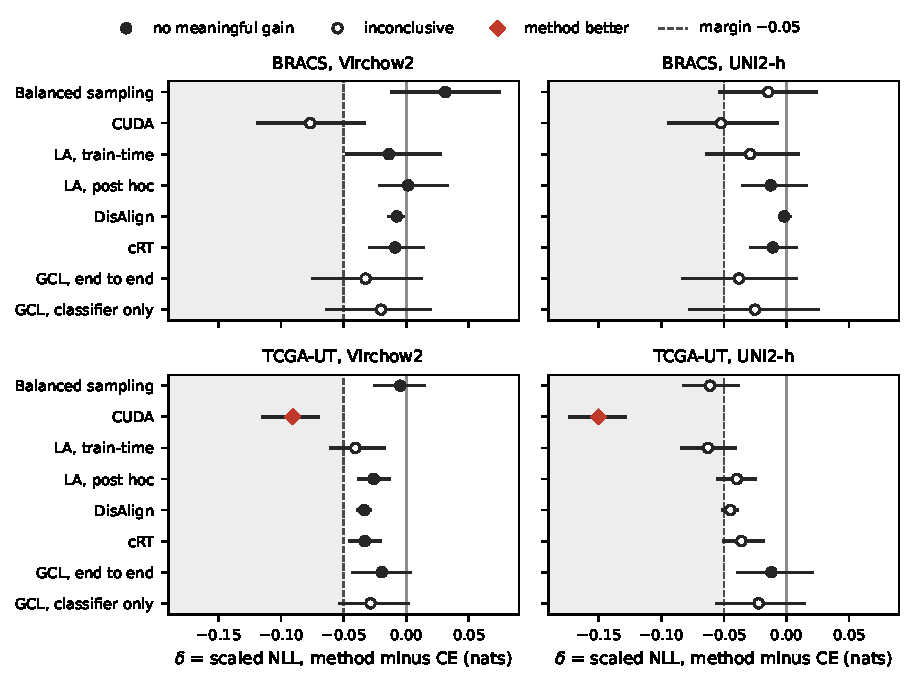
\includegraphics[width=\textwidth]{fig_contrasts.pdf}
\caption{Only CUDA on TCGA-UT improves on temperature-scaled CE by more than the margin. Paired difference $\delta$ in temperature-scaled NLL between each method and CE at $\rho=100$, with 99.84\% intervals (Bonferroni over 32 contrasts); negative values favour the method. The dashed line marks the margin $-0.05$ nats, the solid line zero, and the shaded band meaningful gains. CE: cross-entropy; LA: logit adjustment; CUDA: curriculum of data augmentation; DisAlign: distribution alignment; cRT: classifier re-training; GCL: Gaussian clouded logit adjustment.}
\label{fig:contrasts}
\end{figure}

\begin{table}[htbp]
\centering
\small
\renewcommand{\arraystretch}{1.15}
\begin{tabular}{@{}lrrrr@{}}
\toprule
 & BRACS & BRACS & TCGA-UT & TCGA-UT \\
Method & Virchow2 & UNI2-h & Virchow2 & UNI2-h \\
\midrule
\multicolumn{5}{@{}l}{\emph{Raw NLL minus scaled CE NLL (nats)}} \\
Balanced sampling & $2.19$ & $1.80$ & $0.36$ & $0.30$ \\
CUDA & $0.47$ & $0.46$ & $0.01$ & $-0.06$ \\
LA, train-time & $1.21$ & $1.20$ & $0.16$ & $0.17$ \\
LA, post hoc & $1.15$ & $1.09$ & $0.17$ & $0.17$ \\
DisAlign & $1.51$ & $1.86$ & $0.18$ & $0.22$ \\
cRT & $2.86$ & $2.24$ & $0.41$ & $0.35$ \\
GCL, end to end & $1.73$ & $2.11$ & $0.19$ & $0.55$ \\
GCL, classifier only & $1.93$ & $1.83$ & $0.10$ & $0.20$ \\
\midrule
\multicolumn{5}{@{}l}{\emph{Scaled ECE, method minus CE (points)}} \\
Balanced sampling & $-2.9$ & $-3.7$ & $-0.7$ & $-0.4$ \\
CUDA & $-2.9$ & $-3.4$ & $-1.0$ & $-1.6$ \\
LA, train-time & $-1.2$ & $-1.5$ & $-1.6$ & $-2.2$ \\
LA, post hoc & $0.0$ & $-0.9$ & $-1.7$ & $-2.6$ \\
DisAlign & $-0.5$ & $0.2$ & $-0.7$ & $-0.5$ \\
cRT & $-3.0$ & $-2.9$ & $-1.3$ & $-1.1$ \\
GCL, end to end & $-2.2$ & $-3.1$ & $-1.1$ & $-1.2$ \\
GCL, classifier only & $-2.3$ & $-3.6$ & $-1.9$ & $-1.8$ \\
\bottomrule
\end{tabular}
\caption{Without temperature scaling, no method except CUDA on TCGA-UT comes close to scaled CE; after scaling, almost every method is slightly better calibrated than CE. Point estimates at $\rho=100$ (descriptive). Top: raw NLL of each method minus scaled NLL of CE. Bottom: scaled expected calibration error (ECE) of each method minus that of CE. CE: cross-entropy; LA: logit adjustment; CUDA: curriculum of data augmentation; DisAlign: distribution alignment; cRT: classifier re-training; GCL: Gaussian clouded logit adjustment.}
\label{tab:secondary}
\end{table}


CUDA's two meaningful gains are $-0.091$ nats $[-0.115, -0.070]$ with Virchow2 and $-0.150$ $[-0.173, -0.129]$ with UNI2-h. On BRACS, its intervals exclude zero but not $-0.05$: $-0.077$ $[-0.119, -0.034]$ and $-0.052$ $[-0.094, -0.008]$. The 28 estimates of the other methods lie between $-0.063$ and $0.031$ nats. Fourteen of the 32 intervals lie entirely below zero, eleven of them on TCGA-UT. The largest positive estimate, $0.031$ $[-0.011, 0.074]$, belongs to balanced sampling on BRACS with Virchow2.

The other allocations show the same pattern. At $\rho=50$ and native shares, CUDA's $\delta$ lies between $-0.095$ and $-0.055$ nats, and all its 95\% intervals exclude zero. The other methods lie between $-0.036$ and $0.054$ nats. The only estimate above $0.05$ is balanced sampling at native shares on BRACS with Virchow2, $0.054$ $[0.028, 0.080]$.

Table~\ref{tab:secondary} gives the descriptive comparisons. Without temperature scaling, every method except CUDA has an NLL 1.09 to 2.86 nats above scaled CE on BRACS and 0.10 to 0.55 nats above it on TCGA-UT. CUDA is 0.46 to 0.47 nats above it on BRACS. On TCGA-UT, CUDA matches scaled CE with Virchow2 ($0.01$ $[-0.01, 0.03]$) and lies below it with UNI2-h ($-0.06$ $[-0.08, -0.04]$). After scaling, ECE is lower than CE's for 31 of the 32 comparisons, by up to 3.7 points on BRACS and 2.6 points on TCGA-UT, where scaled CE reaches 12.3 to 14.1 and 3.5 to 5.1 points. All 16 TCGA-UT intervals lie below zero, whereas 7 of the 16 BRACS intervals include it.

\section{Discussion}
\label{sec:discussion}
\textbf{Does any method improve on temperature-scaled CE?} Only CUDA, and only on TCGA-UT. There, its scaled NLL of 0.98 nats with either encoder lies below that of the balanced CE models (1.03), so CUDA does more than undo the imbalance. This agrees with the mitigation studies, in which CUDA also raised the accuracy of the balanced model \citep{queisler2026mitigationTcga}. On BRACS, CUDA points the same way, but its intervals are too wide to show a meaningful gain.

\smallskip\noindent\textbf{Is CUDA's gain a calibration gain?} The data give no sign of it. NLL rewards correct rankings as well as well-calibrated confidence. CUDA's scaled ECE differences fall within the range of the other methods (Table~\ref{tab:secondary}), so its NLL advantage most likely comes from more accurate predictions. This reading is an interpretation; the test does not separate the two sources.

\smallskip\noindent\textbf{What do the inconclusive comparisons mean?} They arise in two ways. On BRACS, both GCL forms with either encoder, and train-time LA and balanced sampling with UNI2-h, have intervals 0.07 to 0.10 nats wide around estimates between $-0.038$ and $-0.015$; the data cannot distinguish a negligible from a moderate gain. With UNI2-h on TCGA-UT, the intervals are narrow, and those of balanced sampling, both forms of LA, cRT, and DisAlign lie entirely below zero, at $-0.063$ to $-0.036$ nats. These methods give a real but small gain, and whether it reaches the margin remains open. On TCGA-UT overall, 11 of 16 intervals exclude zero: after scaling, most methods still lower NLL slightly there.

\smallskip\noindent\textbf{Is a fixed margin of 0.05 nats the right scale?} The margin is absolute: it asks for a 5\% gain in the probability of the true class, whatever the setting. The increase in scaled NLL that imbalance causes, however, ranges from 0.04 to 0.14 nats. On TCGA-UT with Virchow2, the whole increase is smaller than the margin, so a method that fully reversed it would still show no meaningful gain. A check that was not part of the protocol replaces the margin with half of each setting's increase (0.061, 0.072, 0.019, and 0.053 nats). The joint verdict stays the same: 13 contrasts show no meaningful gain, 15 are inconclusive, and 4 show a gain. On TCGA-UT with Virchow2, cRT and DisAlign then join CUDA as better than CE; each removes most of the small increase. The choice of margin therefore decides which methods count as better there, but not the main conclusion. Because the intervals do not depend on the margin, Figure~\ref{fig:contrasts} lets readers apply their own.

\smallskip\noindent\textbf{Can a mitigation method replace temperature scaling?} No. Without scaling, every method except CUDA on TCGA-UT stays at least 0.10 nats above scaled CE. Even CUDA, which has the lowest raw calibration error, remains 6.3 to 8.5 points above the ECE of scaled CE in every setting \citep{queisler2026mitigationBracs,queisler2026mitigationUni2h,queisler2026mitigationTcga,queisler2026mitigationTcgaUni2h}. After scaling, almost every method is slightly better calibrated than CE. In practice, temperature scaling should follow any mitigation method; the method itself is best chosen for accuracy.

\section{Limitations}
\label{sec:limitations}
The test reuses data already inspected in the mitigation studies, whose unpaired intervals motivated it. The protocol was fixed before any contrast was computed, but the test set is not independent. The margin is absolute and not scaled to each setting's imbalance effect; Section~\ref{sec:discussion} shows which decisions depend on it. Bonferroni intervals are conservative, and their bounds rest on about eight replicates each. Eight contrasts have a bound within 0.006 nats of the margin, and their decisions could change with another bootstrap seed. Model selection used balanced accuracy, not NLL, and selecting for calibration could favour other strengths. NLL mixes discrimination and calibration, so a lower NLL does not isolate better calibration. Only $\rho=100$ receives a formal decision; the other allocations are descriptive and missing for UNI2-h on TCGA-UT. Finally, the reference is a single temperature; the test does not evaluate richer post-hoc calibrators, which could narrow CUDA's advantage.

\bibliographystyle{plainnat}
\bibliography{references}
\end{document}
